\section{Method}
Analysing the previously conducted studies, presented in Section \ref{sec:previous_studies}, a couple of conclusions can be drawn. Regarding the setups, the incorporation of a reference instrument allows for a variation of molar fraction that does not demand calculations to find the true molar fraction. Regarding the calibration datasets, studies that vary the molar fraction with the highest frequency seem to obtain datasets with stronger correlation between the K96 output and the molar fraction as well as the environmental parameters.\\

With these conclusions in mind, the following presents, what seems to be, a desired calibration dataset and a setup which one hopefully can produce such a dataset with. Ultimately, a data analysis is presented to ensure the calibration dataset captures what is intended.

\subsection{Calibration dataset}
A general\footnote{In the sense that it captures the essence of the desired calibration dataset, without demanding the data collection to create an exact copy.} desired calibration dataset is presented in Figure \ref{fig:calibration_dataset}. The pressure is varied with the lowest frequency, in steps. At each pressure step, the temperature is varied with a higher frequency, in steps. At each temperature step, the molar fraction is varied with the highest frequency. 

\begin{figure}[htbp]
    \centering
    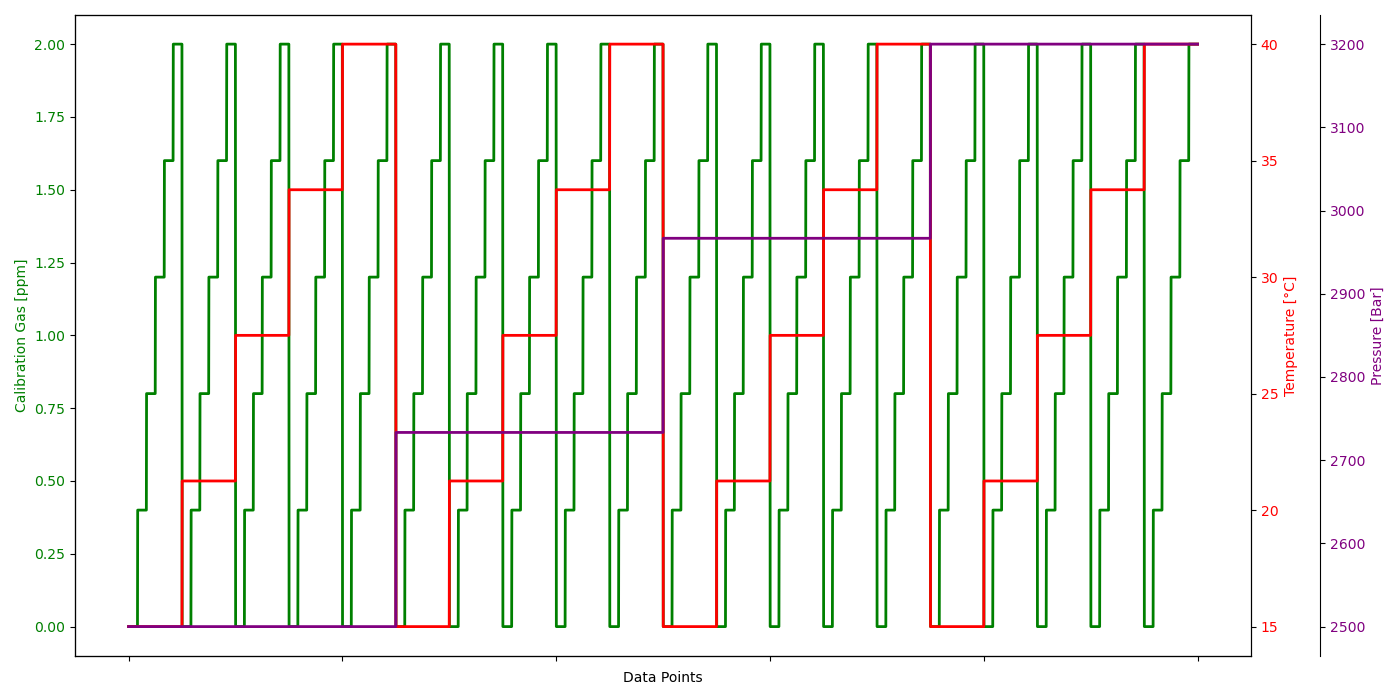
\includegraphics[width=1\linewidth]{figs/method/calibration_dataset.png}
    \caption{Calibration dataset.}
    \label{fig:calibration_dataset}
\end{figure}

The calibration dataset excludes a controlled variation of humidity. The reasoning behind this is that the inclusion of humidity will be hard to realise at the data collection facility\footnote{\href{https://www.icos-sweden.se/norunda}{ICOS SE Norunda research station}}. Also, a significant part of the MIRAGE flight will probably occur during low humidity conditions, due to the dry air at high altitudes.

\subsection{Setup}
A theoretical setup is presented in Figure \ref{fig:setup}.

\begin{figure}[htbp]
    \centering
    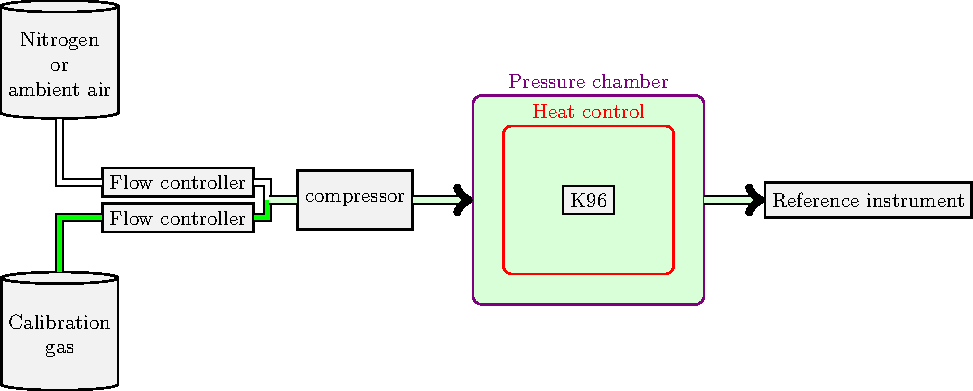
\includegraphics[width=1\linewidth]{figs/method/setup.pdf}
    \caption{Setup.}
    \label{fig:setup}
\end{figure}

Two gas lines are used. One for calibration gas containing methane and carbon dioxide and one for nitrogen gas or ambient air. The flow of each gas line is controlled before the lines are combined into one, enabling control of the molar fraction of the mixed gas. A compressor pressurizes the mixed gas into a pressure chamber, enabling control of the pressure. The pressure chamber possesses a heat control, enabling control of the temperature. The mixed gas is ultimately measured, by the K96 inside the pressure chamber, and by a reference instrument taking the mixed gas from the pressure chamber.

\subsection{Data Analysis}
During data collection, it is important to stop and analyse the data every so often, to ensure it captures what is intended. Therefore, the following presents requirements the calibration dataset must satisfy, and pseudocode that verify if the requirements are satisfied.

\subsubsection*{Requirements}
The requirements the calibration dataset must satisfy are presented in Table \ref{tab:requirements}.

\begin{table}[htbp]
    \centering
    \caption{Calibration dataset requirements.}
    \begin{tabularx}{\textwidth}{cX}
        \toprule
        Requirement & Description\\
        \midrule
        1 & The calibration dataset must capture the effect of the gas molar fraction on the K96 output.\\
        2 & The calibration dataset must capture the effect the environmental parameters on the K96 output.\\
        \bottomrule
    \end{tabularx}
    \label{tab:requirements}
\end{table}

The purpose of MIRAGE is to measure methane and carbon dioxide. Therefore requirement 1 ensures the calibration dataset captures the effects of the gases on the K96 output. The purpose of the calibration is to mitigate the unwanted effects of the environmental parameters on the K96 output. Therefore requirement 2 ensures the calibration dataset captures such unwanted effects.

\subsubsection*{Pseudocode}
The pseudocode that verify if the requirements are satisfied is presented in Listings \ref{lst:import}, \ref{lst:corr} and \ref{lst:scatter}.

\begin{lstlisting}[caption=Imports., label=lst:import]
import pandas as pd
import matplotlib.pyplot as plt

df = pd.read_csv("calibration_dataset.csv")
\end{lstlisting}

Listing \ref{lst:import} imports the required libraries and reads the calibration dataset, provided in a csv file.

\begin{lstlisting}[caption=Correlation matrix., label=lst:corr]
print(df[['gas_molar_fraction', 'environmental_parameters', 'k96_output']].corr())
\end{lstlisting}

Listing \ref{lst:corr} computes pairwise correlation between the gas molar fraction, the environmental parameters and the K96 output, and returns a correlation matrix.

\begin{lstlisting}[caption=Correlation scatter plots., label=lst:scatter]
fig, (ax1, ax2) = plt.subplots(1, 2)

ax1.scatter(df['gas_molar_fraction'], df['k96_output'], alpha=0.3)
ax1.set_xlabel('gas_molar_fraction [ppm]')
ax1.set_ylabel('k96_output')

ax2.scatter(df['environmental_parameters'], df['k96_output'], alpha=0.3)
ax2.set_xlabel('environmental_parameters')
ax2.set_ylabel('k96_output')

plt.tight_layout()
plt.show()
\end{lstlisting}

Listing \ref{lst:scatter} returns scatter plots of the gas molar fraction vs the K96 output and the environmental parameters vs the K96 output.